\section{Week Schedule - Border Around Pictograms}
\userstory{As a user, I would like to have pictograms shown with a surrounding border, such that they are clearly distinguished from the background.}
This task was taken after the initial planning therefore it has not been does not have an estimated amount of EP. 
This task was given a \phigh-priority by the product owner. 

In the Week Schedule application it can be hard to distinguish between pictrograms and the background.
Mostly pictograms with a white background and Sunday's background, which is white as can be seen on \myref{fig:before-after-borders}.

Changing the background colour of a weekday is not possible since the colours are predefined by the costumer, such that they represent the current physical version of week schedules in use.

To solve this issue a border will be drawn around each pictogram in Week Schedule.
Currently the pictograms exists as squares, but are rounded with a radius of 10 pixels.
To draw a border along the edge of the image, it needs to follow the same path as the rounded pictogram. 
To implement this we add the drawing of this to the \texttt{onDraw()} method of the \texttt{RoundedImageView} class which renders the pictogram inside the Week Schedule application. 
Since the same border will be needed for each pictogram, we use the singleton pattern to make it once and reuse the same object as argument for the method call which draws the image on the screen. 
We refactor the old code to do the same for the rounded corners. 

This change will also reduce the number of allocations, and  thusly helps to reduce the number of garbage collection pauses, which can freeze the system\footnote{\url{http://developer.android.com/training/articles/perf-tips.html\#ObjectCreation}}. 
Since other methods also uses the \texttt{RoundedImageView} class the singleton should change if called with different dimensions as it requires different rounded edges and borders. 
In this case the objects should be corrected to fit the new dimensions. 

An example of one of the singletons is shown in \myref{lst:singleton_example}.
The result of these changes is show in \myref{fig:before-after-borders}. 

\begin{lstlisting}[float, floatplacement=h, caption={One of the singletons used to solve this task.}, label={lst:singleton_example}] 
private static Path drawPath;

/**
 * Creates and/or gets the Path used to draw the border around the pictograms with rounded corners.
 * Using the singleton pattern.
 * @param roundedImageView The imageview(pictogram) which the path will be used on.
 * @param cornerRadius The radius of the rounded corner.
 * @param borderWidth Width of the border.
 * @return The path used for drawing the border around the pictograms.
 */
public static Path getDrawPath(RoundedImageView roundedImageView, float cornerRadius, float borderWidth){
    if(drawPath == null)
        drawPath = new Path();
    if(roundedImageView.getHeight() != drawPathHeight) {
        drawPath.reset();
        drawPathHeight = roundedImageView.getHeight();
        RectF rectf = new RectF(borderWidth, borderWidth,
                roundedImageView.getWidth() - borderWidth, roundedImageView.getHeight() - borderWidth);
        drawPath.addRoundRect(rectf, cornerRadius - borderWidth,
                cornerRadius - borderWidth, Path.Direction.CW);
    }
    return drawPath;
}
\end{lstlisting} 

\begin{figure*}[h]
    \centering
        \begin{subfigure}[t]{0.5\textwidth}
        \centering
        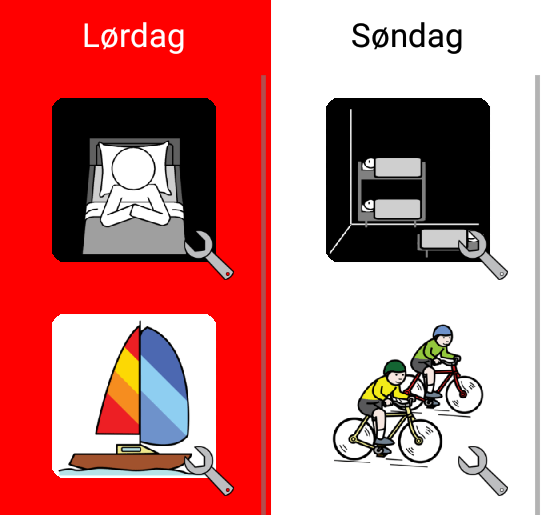
\includegraphics[width=0.6\textwidth]{figures/img/screenshots/old_week_schedule_no_borders.png}
        \caption{Without borders}
    \end{subfigure}\hfill
        \begin{subfigure}[t]{0.5\textwidth}
        \centering
        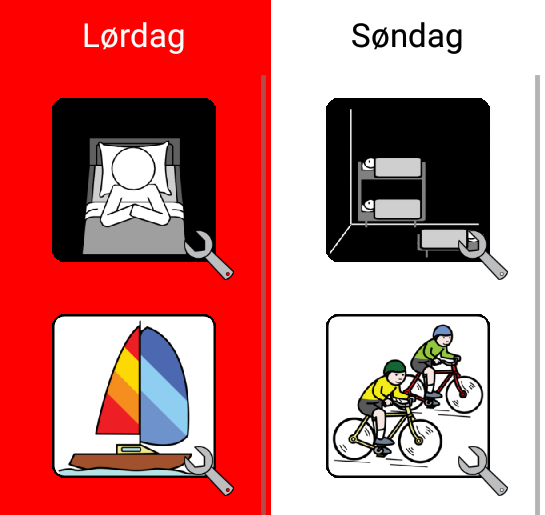
\includegraphics[width=0.6\textwidth]{figures/img/screenshots/new_week_schedule_with_borders.png}
        \caption{With borders}
    \end{subfigure}
    \caption{Comparison of the pictograms in the Week Schedule application before and after adding a border.}
    \label{fig:before-after-borders}
\end{figure*}

Implementing and testing these changes took 3 EP. 
